\documentclass[expanded]{lkx_pset}

\title{CS181 Problem Set 6}
\author{Lev Kruglyak}
\due{April 26, 2024}

\usepackage{pgfplots}
\pgfplotsset{compat=1.14}
\usepackage[outputdir=build]{minted}
\usepackage{graphicx}

\usepackage{amsmath}
\usepackage{amssymb}
\usepackage{graphicx}
\usepackage{tikz}
\usetikzlibrary{patterns}
\usepackage{subfig}
\usepackage{comment}

\newcommand{\boldA}{\mathbf{A}}
\newcommand{\boldB}{\mathbf{B}}
\newcommand{\boldC}{\mathbf{C}}
\newcommand{\boldD}{\mathbf{D}}
\newcommand{\boldE}{\mathbf{E}}
\newcommand{\boldF}{\mathbf{F}}
\newcommand{\boldG}{\mathbf{G}}
\newcommand{\boldH}{\mathbf{H}}
\newcommand{\boldI}{\mathbf{I}}
\newcommand{\boldJ}{\mathbf{J}}
\newcommand{\boldK}{\mathbf{K}}
\newcommand{\boldL}{\mathbf{L}}
\newcommand{\boldM}{\mathbf{M}}
\newcommand{\boldN}{\mathbf{N}}
\newcommand{\boldO}{\mathbf{O}}
\newcommand{\boldP}{\mathbf{P}}
\newcommand{\boldQ}{\mathbf{Q}}
\newcommand{\boldR}{\mathbf{R}}
\newcommand{\boldS}{\mathbf{S}}
\newcommand{\boldT}{\mathbf{T}}
\newcommand{\boldU}{\mathbf{U}}
\newcommand{\boldV}{\mathbf{V}}
\newcommand{\boldW}{\mathbf{W}}
\newcommand{\boldX}{\mathbf{X}}
\newcommand{\boldY}{\mathbf{Y}}
\newcommand{\boldZ}{\mathbf{Z}}
\newcommand{\bolda}{\mathbf{a}}
\newcommand{\boldb}{\mathbf{b}}
\newcommand{\boldc}{\mathbf{c}}
\newcommand{\boldd}{\mathbf{d}}
\newcommand{\bolde}{\mathbf{e}}
\newcommand{\boldf}{\mathbf{f}}
\newcommand{\boldg}{\mathbf{g}}
\newcommand{\boldh}{\mathbf{h}}
\newcommand{\boldi}{\mathbf{i}}
\newcommand{\boldj}{\mathbf{j}}
\newcommand{\boldk}{\mathbf{k}}
\newcommand{\boldl}{\mathbf{l}}
\newcommand{\boldm}{\mathbf{m}}
\newcommand{\boldn}{\mathbf{n}}
\newcommand{\boldo}{\mathbf{o}}
\newcommand{\boldp}{\mathbf{p}}
\newcommand{\boldq}{\mathbf{q}}
\newcommand{\boldr}{\mathbf{r}}
\newcommand{\bolds}{\mathbf{s}}
\newcommand{\boldt}{\mathbf{t}}
\newcommand{\boldu}{\mathbf{u}}
\newcommand{\boldv}{\mathbf{v}}
\newcommand{\boldw}{\mathbf{w}}
\newcommand{\boldx}{\mathbf{x}}
\newcommand{\boldy}{\mathbf{y}}
\newcommand{\boldz}{\mathbf{z}}

\newcommand{\mcA}{\mathcal{A}}
\newcommand{\mcB}{\mathcal{B}}
\newcommand{\mcC}{\mathcal{C}}
\newcommand{\mcD}{\mathcal{D}}
\newcommand{\mcE}{\mathcal{E}}
\newcommand{\mcF}{\mathcal{F}}
\newcommand{\mcG}{\mathcal{G}}
\newcommand{\mcH}{\mathcal{H}}
\newcommand{\mcI}{\mathcal{I}}
\newcommand{\mcJ}{\mathcal{J}}
\newcommand{\mcK}{\mathcal{K}}
\newcommand{\mcL}{\mathcal{L}}
\newcommand{\mcM}{\mathcal{M}}
\newcommand{\mcN}{\mathcal{N}}
\newcommand{\mcO}{\mathcal{O}}
\newcommand{\mcP}{\mathcal{P}}
\newcommand{\mcQ}{\mathcal{Q}}
\newcommand{\mcR}{\mathcal{R}}
\newcommand{\mcS}{\mathcal{S}}
\newcommand{\mcT}{\mathcal{T}}
\newcommand{\mcU}{\mathcal{U}}
\newcommand{\mcV}{\mathcal{V}}
\newcommand{\mcW}{\mathcal{W}}
\newcommand{\mcX}{\mathcal{X}}
\newcommand{\mcY}{\mathcal{Y}}
\newcommand{\mcZ}{\mathcal{Z}}

\newcommand{\reals}{\ensuremath{\mathbb{R}}}
\newcommand{\integers}{\ensuremath{\mathbb{Z}}}
\newcommand{\rationals}{\ensuremath{\mathbb{Q}}}
\newcommand{\naturals}{\ensuremath{\mathbb{N}}}
\newcommand{\trans}{\ensuremath{\mathsf{T}}}
\newcommand{\ident}{\mathbf{I}}
\newcommand{\bzero}{\mathbf{0}}

\newcommand{\balpha}{\mathbf{\alpha}}
\newcommand{\bbeta}{\mathbf{\beta}}
\newcommand{\bdelta}{\mathbf{\delta}}
\newcommand{\boldeta}{\mathbf{\eta}}
\newcommand{\bkappa}{\mathbf{\kappa}}
\newcommand{\bgamma}{\mathbf{\gamma}}
\newcommand{\bmu}{\boldsymbol{\mu}}
\newcommand{\bphi}{\mathbf{\phi}}
\newcommand{\bpi}{\boldsymbol{\pi}}
\newcommand{\bpsi}{\mathbf{\psi}}
\newcommand{\bsigma}{\mathbf{\sigma}}
\newcommand{\btheta}{\mathbf{\theta}}
\newcommand{\bxi}{\mathbf{\xi}}
\newcommand{\bGamma}{\mathbf{\Gamma}}
\newcommand{\bLambda}{\mathbf{\Lambda}}
\newcommand{\bOmega}{\mathbf{\Omega}}
\newcommand{\bPhi}{\mathbf{\Phi}}
\newcommand{\bPi}{\mathbf{\Pi}}
\newcommand{\bPsi}{\mathbf{\Psi}}
\newcommand{\bSigma}{\mathbf{\Sigma}}
\newcommand{\bTheta}{\mathbf{\Theta}}
\newcommand{\bUpsilon}{\mathbf{\Upsilon}}
\newcommand{\bXi}{\mathbf{\Xi}}
\newcommand{\bepsilon}{\mathbf{\epsilon}}

\def\argmin{\operatornamewithlimits{arg\,min}}

\newcommand{\given}{\,|\,}
\newcommand{\distNorm}{\mathcal{N}}

\newcommand{\mueps}{\mu_{\epsilon}}
\newcommand{\sigeps}{\sigma_{\epsilon}}
\newcommand{\mugam}{\mu_{\gamma}}
\newcommand{\siggam}{\sigma_{\gamma}}
\newcommand{\muzp}{\mu_{p}}
\newcommand{\sigzp}{\sigma_{p}}
\newcommand{\gauss}[3]{\frac{1}{2\pi#3}e^{-\frac{(#1-#2)^2}{2#3}}}


\usetikzlibrary{bayesnet}

% \collaborator{Artemas Radik}
% \collaborator{Leonardo Kaplan}
\collaborator{AJ LaMotta}
\collaborator{GPT-4 (for debugging help)}

\begin{document}
\maketitle

\begin{problem}{1}[Hidden Markov Models]
In this problem, you will be working with one-dimensional Kalman filters, which are \textit{continuous-state} Hidden Markov Models. Let $z_0, z_1, \cdots , z_T$ be the hidden states of the system and $x_0, x_1, \cdots, x_T$ be the observations produced. Then, state transitions and emissions of observations work as follows:
\begin{eqnarray*}
	z_{t+1} &= z_{t} + \epsilon_{t} \\
	x_{t} & = z_{t} + \gamma_{t}
\end{eqnarray*}
where $\epsilon_t \sim N(0,\sigeps^2)$ and $\gamma_t \sim N(0,\siggam^2)$. The value of the first hidden state follows the distribution $z_0 \sim N(\muzp,\sigzp^2)$.
\end{problem}
\begin{parts}
	\begin{part}{1} Draw the graphical model corresponding to the one-dimensional Kalman filter.
	\end{part}

	The graphical model is:

	\begin{center}
		\begin{tikzpicture}
			\node[latent] (z0) {$\mathbf{z}_0$};%
			\node[latent, right=of z0] (z1) {$\mathbf{z}_1$};%
			\node[const, right=of z1] (dots) {$\;\cdots\;$};%
			\node[latent, right=of dots] (zT) {$\mathbf{z}_T$};%

			\node[obs, below=of z0] (x0) {$\mathbf{x}_0$};%
			\node[obs, below=of z1] (x1) {$\mathbf{x}_1$};%
			\node[obs, below=of zT] (xT) {$\mathbf{x}_T$};%

			\edge {z0} {x0}
			\edge {z1} {x1}
			\edge {zT} {xT}

			\edge {z0} {z1}
			\edge {z1} {dots}
			\edge {dots} {zT}
		\end{tikzpicture}
	\end{center}

	\begin{part}{2} In this part we will walk through the derivation of the conditional distribution of $z_t|(x_0, \cdots, x_{t})$.
	\end{part}
	\begin{parts}
		\begin{part}{a} How does the quantity $p(z_t| x_0, \cdots, x_{t})$ relate to $\alpha_t(z_t)$ and $\beta_t(z_t)$ from the forward-backward algorithm for HMMs?  What is the operation we are performing called?
		\end{part}

		The operation is often called \emph{filtering} for discrete HMMs, and defining
		\[
			\begin{aligned}
				\alpha_t(z_t = z) & = p(x_1,\ldots, x_t, z_t = z),         \\
				\beta_t(z_t = z)  & = p(x_{t+1},\ldots, x_T \mid z_t = z),
			\end{aligned}
		\]
		we the relation $p(z_t\mid x_0, \ldots, x_t) \propto \alpha_t(z_t)$ by Bayes rule.

		\begin{part}{b} The above quantity $p(z_t|x_0, \cdots, x_t)$ is the PDF for a Normal distribution with mean $\mu_t$ and variance $\sigma_t^2$. We start our derivation of $\mu_t$ and $\sigma_t^2$ by writing:
			\begin{align*}
				p(z_t|x_0, \cdots, x_t) \propto p(x_t|z_t)p(z_t|x_0, \cdots x_{t-1})
			\end{align*}
			What is $p(x_t|z_t)$ equal to?
		\end{part}

		Notice that the marginal distribution $x_t\mid z_t \sim \mathcal{N}(z_t, \sigma_\gamma^2)$, so we can expand
		\[
			p(x_t\mid z_t) = \mathcal{N}(x_t; z_t, \sigma^2_\gamma) = \frac{1}{\sigma_\gamma \sqrt{2\pi}}\exp\left( -\frac{1}{2\sigma_\gamma^2}(x_t -z_t)^2\right).
		\]

		\begin{part}{c} Suppose we are given the mean and variance of the conditional distribution $z_{t-1}|(x_0, \cdots, x_{t-1})$ as $\mu_{t-1}$, $\sigma^2_{t-1}$. What is $p(z_t|x_0, \cdots x_{t-1})$ equal to?
		\end{part}

		Marginalizing out over $z_{t-1}$ gives us
		\[
			p(z_t\mid x_0, \ldots, x_{t-1}) = \int_{-\infty}^\infty p(z_{t-1} \mid x_0, \ldots, x_{t-1})\, p(z_t\mid x_0,\ldots, x_{t-1}, z_{t-1} \,dz_{t-1}.
		\]
		Then since we know that $p(z_{t-1}\mid x_0,\ldots, x_{t-1}) = \mathcal{N}(z_{t-1};\mu_{t-1}, \sigma^2_{t-1})$, and that $z_t \perp (x_0,\ldots, x_{t-1})\mid z_{t-1}$, we get
		\[
			p(z_t \mid x_0, \ldots, x_{t-1}, z_{t-1}) = p(z_t\mid z_{t-1}) = \mathcal{N}(z_t; z_{t-1}, \sigma_\epsilon^2) = \mathcal{N}(z_t - z_{t-1}; 0, \sigma^2_\epsilon).
		\]
		Now using the fact that
		\[\int \mathcal{N}(y-x ; \mu_a, \sigma^2_a)\mathcal{N}(x ; \mu_b, \sigma^2_b)\,dx = \mathcal{N}(y ; (\mu_a + \mu_b), (\sigma^2_a + \sigma^2_b)),\]
		we get the expression:
		\[
			p(z_t\mid x_0,\ldots, x_{t-1}, z_{t-1})
			= \int_{-\infty}^\infty \mathcal{N}(z_T - x; 0, \sigma_\epsilon^2) \mathcal{N}(x; \mu_{t-1},\sigma_{t-1}^2)\,dx.
		\]

		\begin{part}{d} Combine your answers from parts (b) and (c) to get a final expression for $p(z_t|x_0, \cdots, x_t)$. Report the mean $\mu_t$ and variance $\sigma_t^2$ of this Normal.
		\end{part}

		Finally, combining the previous parts we get the expansion
		\[
			p(z_t\mid x_0, \ldots, x_t) = \mathcal{N}(x_t; z_t,\sigma_\gamma^2)\mathcal{N}(z_t; \mu_{t-1}, \sigma_{t-1}^2 + \sigma_\epsilon^2)=\mathcal{N}(z_t; \mu_t, \sigma_t^2),
		\]
		where we have
		\[
			\mu_t = \frac{\sigma^2_{t-1}+\sigma^2_\epsilon}{\sigma^2_{t-1} + \sigma_\epsilon^2 + \sigma_\gamma^2}x_t + \frac{\sigma^2_\gamma}{\sigma^2_{t-1}+\sigma_\epsilon^2 + \sigma_\gamma^2}\mu_{t-1},\quad \sigma^2_t = \left(\frac{1}{\sigma^2_{t-1} + \sigma_\epsilon^2} + \frac{1}{\sigma_\gamma^2}\right)^{-1}.
		\]
	\end{parts}
	\begin{part}{3}Interpret $\mu_t$ in terms of how it combines observations from the past with the current observation.
	\end{part}

	Note that $\mu_t$, our prediction for the current sample, is a weighted average of $x_t$, our current observation, and $\mu_{t-1}$, which is our prediction from the previous samples. The weights in this weighted sum are not just constant, but depend on $\sigma_{t-1}^2$ which represents the uncertainty in the previous predictions.
\end{parts}

\begin{problem}{2}[Policy and Value Iteration]
You have a robot that you wish to collect two parts in an environment
and bring them to a goal location.  There are also parts of the
environment that you wish the robot avoid to reduce wear on the floor.
Eventually, you settle on the following way to model the environment
as a Gridworld.  The ``states'' in Gridworld are represented by
locations in a two-dimensional space.  Here we show each state and its
reward:
\end{problem}

\begin{solution}
	\begin{center}
		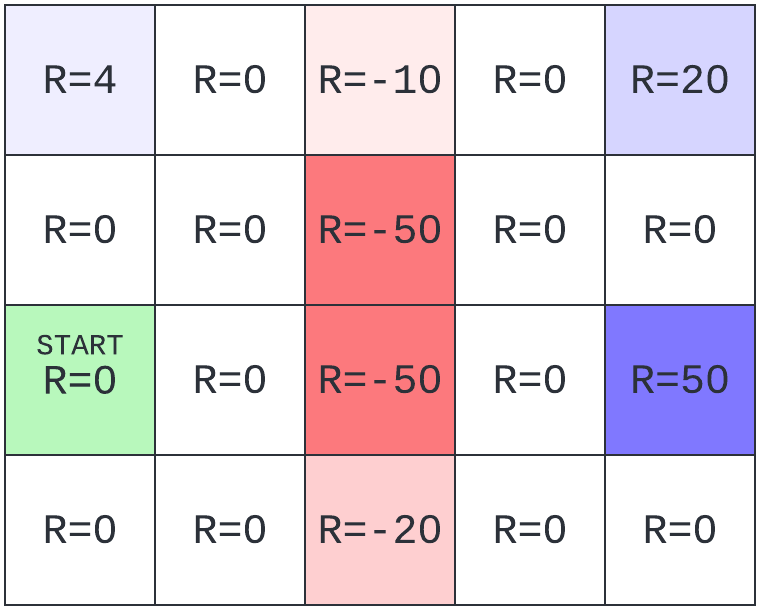
\includegraphics[width=3in]{images/gridworld.png}
	\end{center}

	The set of actions is \{N, S, E, W\}, which corresponds to moving north (up), south (down), east (right), and west (left) on the grid. Taking an action in Gridworld does not always succeed with probability
	$1$; instead the agent has probability $0.1$ of ``slipping'' into a
	state on either side, but not backwards.  For example, if the agent tries to move right from START, it succeeds with probability 0.8, but the agent may end up moving up or down with probability 0.1 each. Also, the agent cannot move off the edge of the grid, so moving left from START will keep the agent in the same state with probability 0.8, but also may slip up or down with probability 0.1 each. Lastly, the agent has no chance of slipping off the grid - so moving up from START results in a 0.9 chance of success with a 0.1 chance of moving right.

	Also, the agent does not receive the reward of a state immediately upon entry, but instead only after it takes an action at that state. For example, if the agent moves right four times (deterministically, with no chance of slipping) the rewards would be +0, +0, -50, +0, and the agent would reside in the +50 state. Regardless of what action the agent takes here, the next reward would be +50.

	In this problem, you will first implement policy and value iteration in this setting and discuss the policies that you find.  Next, you will interrogate whether this approach to modeling the original problem was appropriate.

	Your job is to implement the following three methods in file \texttt{homework6.ipynb}. Please use the provided helper functions \texttt{get\_reward} and \texttt{get\_transition\_prob} to implement your solution.

	Note that we are doing infinite-horizon planning to maximize the expected reward of the traveling agent. For parts 1-3, set discount factor $\gamma = 0.7$.

	\newpage
	\begin{part}{1a}
		Implement function \texttt{policy\_evaluation}.  Your
		solution should learn value function $V$, either using a closed-form expression or iteratively using
		convergence tolerance $\texttt{theta = 0.0001}$ (i.e., if
		$V^{(t)}$ represents $V$ on the $t$-th iteration of your policy
		evaluation procedure, then if $|V^{(t + 1)}[s] - V^{(t)}[s]|
			\leq \theta$ for all $s$, then terminate and return $V^{(t + 1)}$.)
	\end{part}

	Using the closed form expression for $V$, we get the following code:
	\begin{minted}{python}
	def policy_evaluation(pi, gamma):
    	R = np.array([get_reward(i) for i in range(num_states)]).reshape(-1, 1)
    	T = np.array([
    		  [get_transition_prob(i, pi[i], j) 
    		  for j in range(num_states)] for i in range(num_states)
    	  ])

    	return (np.linalg.inv(np.eye(num_states) - gamma * T) @ R).flatten()
  \end{minted}

	\begin{part}{1b}
		Implement function \texttt{update\_policy\_iteration} to update the policy \texttt{pi} given a value function \texttt{V} using \textbf{one step} of policy iteration.
	\end{part}

	The code is:
	\begin{minted}{python}
	def update_policy_iteration(V, gamma):
    	pi_new = np.zeros(num_states)

    	for s in range(num_states):
        	T = np.array([
        	  [get_transition_prob(s, i, j) for j in range(num_states)] 
        	  for i in range(4)
        	])
        	Q = get_reward(s) + gamma * (T @ V)
        	pi_new[s] = np.argmax(Q)

    	return pi_new
	\end{minted}

	\newpage
	\begin{part}{1c}
		Set \texttt{max\_iter = 4}, \texttt{print\_every = 1} to show the learned value function and the associated policy for the first 4 policy iterations. Do not modify the plotting code. Please fit all 4 plots onto one page of your writeup.
	\end{part}

	\begin{center}
		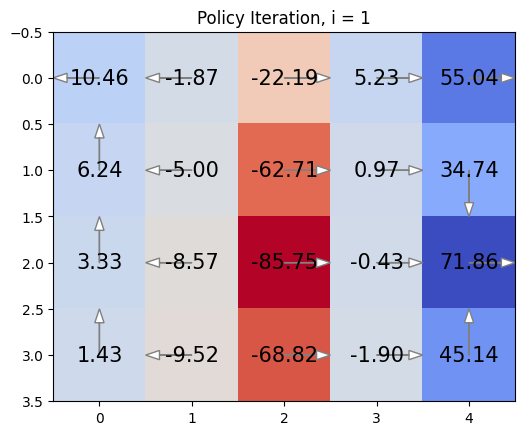
\includegraphics[scale=0.5]{figures/1c-1.png}
		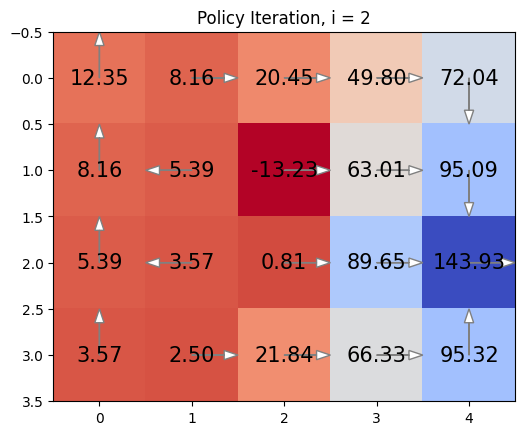
\includegraphics[scale=0.5]{figures/1c-2.png}
		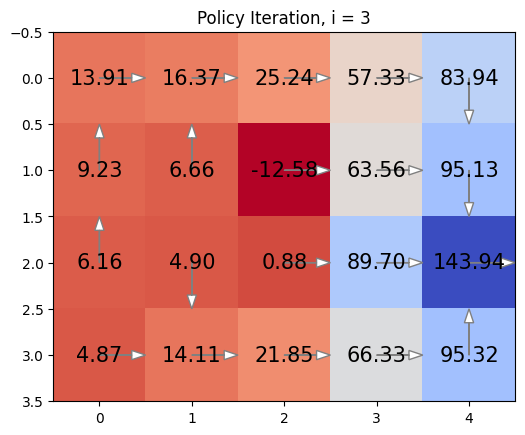
\includegraphics[scale=0.5]{figures/1c-3.png}
		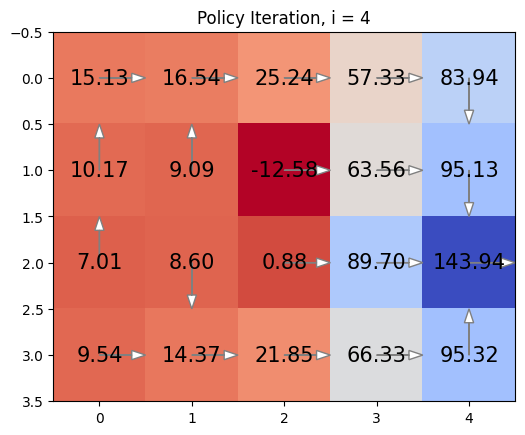
\includegraphics[scale=0.5]{figures/1c-4.png}
	\end{center}

	\begin{part}{1d} Set \texttt{ct = 0.01} and increase \texttt{max\_iter} such that the algorithm converges. Include a plot of the final learned value function and policy. How many iterations does it take to converge? Now try \texttt{ct = 0.001} and \texttt{ct = 0.0001}. How does this affect the number of iterations until convergence?
	\end{part}

	It takes $5$ iterations to converge for $\texttt{ct = 0.01}$, and here is the final learned value function:
	\begin{center}
		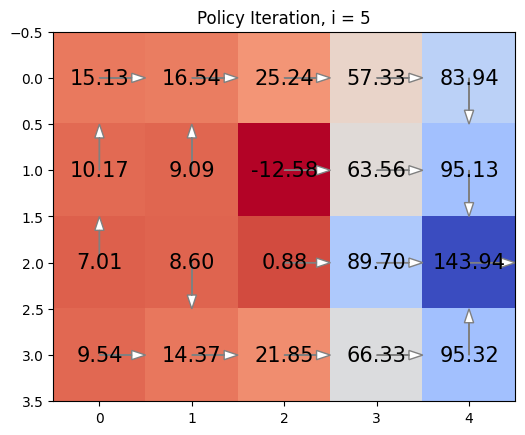
\includegraphics[scale=0.5]{figures/1d.png}
	\end{center}
	For $\texttt{ct = 0.001}$ and $\texttt{ct = 0.0001}$ we get the same results -- $5$ iterations to converge.

	\begin{part}{2a} Implement function
		\texttt{update\_value\_iteration}, which performs \textbf{one step} of value iteration to update \texttt{V}, \texttt{pi}.
	\end{part}

	Here is the code:
	\begin{minted}{python}
	def update_value_iteration(V, pi, gamma):
    	V_new = np.zeros(num_states)
    	pi_new = np.zeros(num_states)
    	
    	T = [np.array([[get_transition_prob(s, i, j) for j in
        	range(num_states)] for i in range(4)]) for s in
        	range(num_states)]

    	for s in range(num_states):
        	Q = get_reward(s) + gamma * (T[s] @ V)
        	V_new[s] = np.max(Q)

    	for s in range(num_states):
        	Q = get_reward(s) + gamma * (T[s] @ V_new)
        	pi_new[s] = np.argmax(Q)

    	return V_new, pi_new
	\end{minted}

	\begin{part}{2b} Set \texttt{max\_iter = 4}, \texttt{print\_every = 1} to show the learned value function and the associated policy for the first 4 value iterations. Do not modify the plotting code. Please fit all 4 plots onto one page of your writeup.
	\end{part}

	\begin{center}
		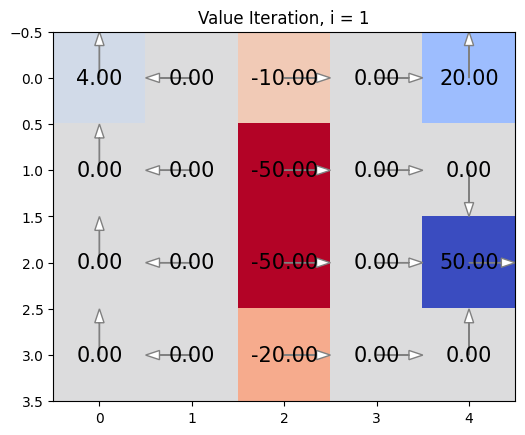
\includegraphics[scale=0.5]{figures/2b-1.png}
		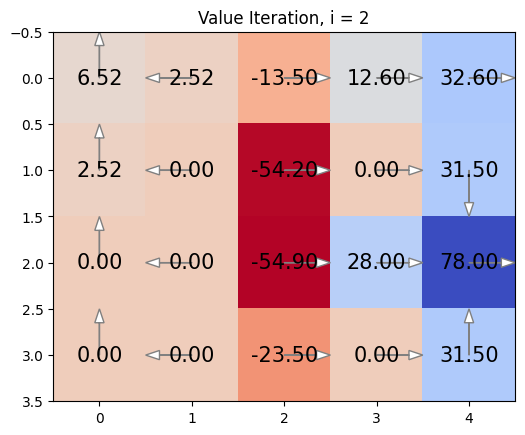
\includegraphics[scale=0.5]{figures/2b-2.png}
		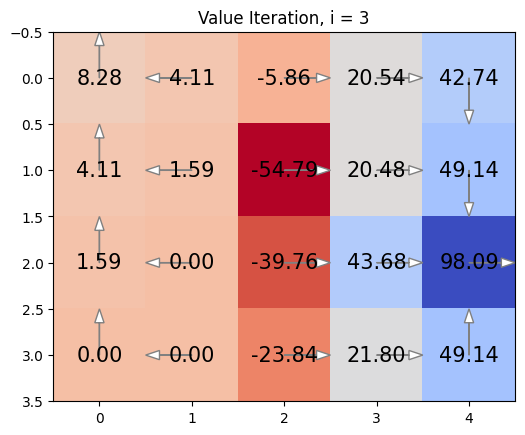
\includegraphics[scale=0.5]{figures/2b-3.png}
		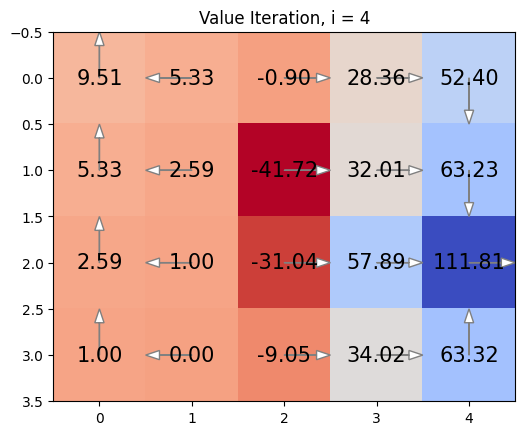
\includegraphics[scale=0.5]{figures/2b-4.png}
	\end{center}

	\begin{part}{2c} Set \texttt{ct = 0.01} and increase \texttt{max\_iter} such that the algorithm converges. Include a plot of the final learned value function and policy. How many iterations does it take to converge? Now try \texttt{ct = 0.001} and \texttt{ct = 0.0001}. How does this affect the number of iterations until convergence?
	\end{part}

	It takes $25$ iterations to converge for $\texttt{ct = 0.01}$, and here is the final learned value function:
	\begin{center}
		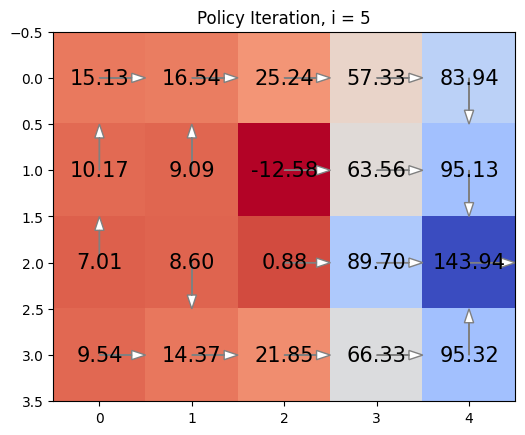
\includegraphics[scale=0.5]{figures/1d.png}
	\end{center}
	For $\texttt{ct = 0.001}$ and $\texttt{ct = 0.0001}$ it takes $31$ and $38$ iterations to converge respectively.

	\begin{part}{3} Compare and contrast the number of iterations, time per iteration, and overall runtime between policy iteration and value iteration. What do you notice?
	\end{part}

	Policy iteration converged in far fewer iterations that value iteration, but took a comparable amount of time, meaning that a single policy iteration takes a longer. It's difficult to get an exact, reliable benchmark for this in Python since they both take a bit less than a second to run.

	\begin{part}{4} Plot the learned policy with each of $\gamma \in (0.6,0.7,0.8,0.9)$. Include all 4 plots in your writeup. Describe what you see and provide explanations for the differences in the observed policies. Also discuss the effect of gamma on the runtime for both policy and value iteration.
	\end{part}

	Ordered from left to right in terms of increasing $\gamma$, we get the following plots:
	\begin{center}
		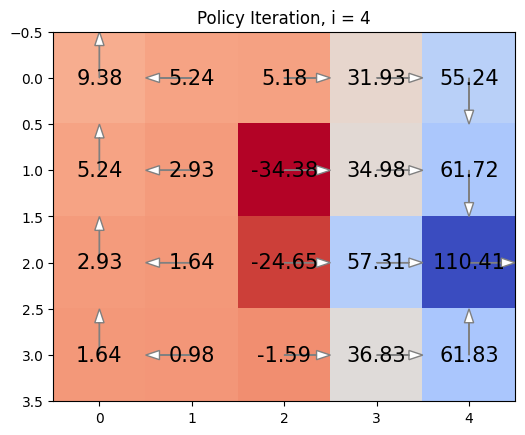
\includegraphics[scale=0.5]{figures/4-1.png}
		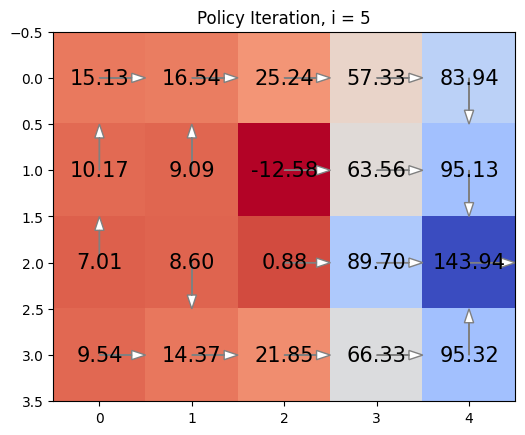
\includegraphics[scale=0.5]{figures/4-2.png}
		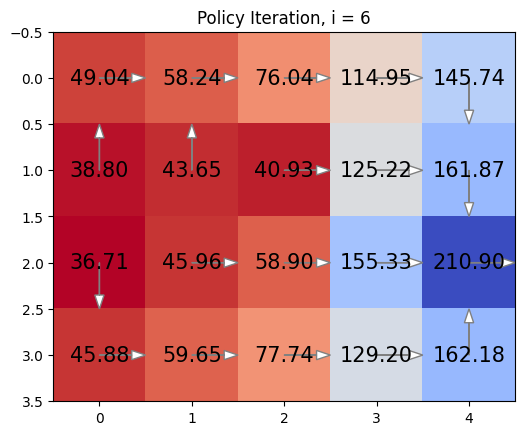
\includegraphics[scale=0.5]{figures/4-3.png}
		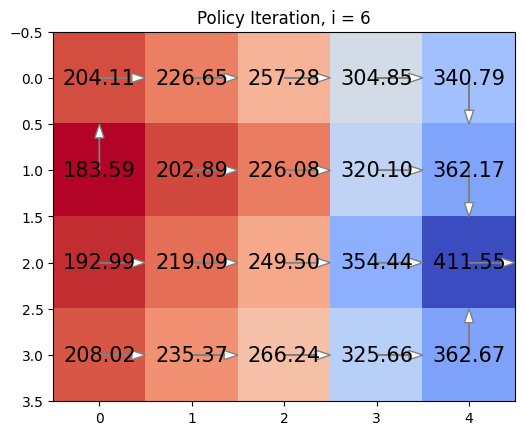
\includegraphics[scale=0.5]{figures/4-4.png}
	\end{center}
	First of all, it's clear that as $\gamma$ increased, the learned value for each grid cell increase. This is a direct consequence of the formula for updating value -- with a higher $\gamma$, there is an increased reward for future actions. Secondly, and more importantly, increasing $\gamma$ seems to lead to the optimal policy ignoring negative rewards, and instead making a beeline straight for the biggest reward. This can be seen explicitly: For $\gamma=0.6$, the worst valued cells are the ones with the lowest reward, however for $\gamma=0.9$ the worst valued cells are the ones which are farthest from the maximal reward.

	\begin{part}{5} Now suppose that the game ends at any state with a positive reward, i.e. it immediately transitions you to a new state with zero reward that you cannot transition away from. What do you expect the optimal policy to look like, as a function of gamma? Numerical answers are not required, intuition is sufficient.
	\end{part}

	When $\gamma$ is low, future rewards will be heavily discounted so the agent will try to reach a positive reward as quickly as possible while dodging any negative rewards along the way. If there is a nearby positive reward, it might prioritize getting to it as soon as possible, even ending the game here, instead of trying to manouver around negative rewards and getting to a larger positive reward further away.

	When $\gamma$ is high, the agent places similar value on immediate and distant future rewards, so the agent will try reach the distant reward, potentially sacrificing some points to get there. It will be more avoidant of the negative reward and try to get to the farther away bigger rewards. In between the extremes, there is a tradeoff based on the $\gamma$ factor.

	\begin{part}{}
		Now you will interrogate your solution in terms of its applicability
		for the intended task of picking up two objects and bringing them to a
		goal location.
	\end{part}

	\begin{part}{6} In this problem, we came up with a model for the problem,
		solved it, and then we had a policy to use on the real robot.  An
		alternative could have been to use RL on the robot to identify a
		policy that achieved your objective.  What is the value of the
		approach we took?  What are some limitations (in general)?
	\end{part}

	The advantage of our modelling approach is that we only have to do a single pass of value or policy iteration until convergence, then we have an optimal policy. With a reinforcement learning approach, especially in an unknown search space, there aren't such convergence guarantees. A big limitation of this approach would be if the environment was too complex to be modelled, or changing with time. In this event, reinforcement learning would be advantageous. Another limitation is that the agent never directly interact with the true environment, so there is no guarantee that it would work effectively once the assumptions of the model would be removed.


	\begin{part}{7} Do any of the policies learned actually accomplish the task
		that you desired?  What modeling shortcuts were made that result
		in some policies matching your true objective and some not?
	\end{part}

	Some of the learned policies accomplish the goal, especially the one learned by policy iteration. In value iteration, the optimal policy gets stuck at the first part. This represents a modelling failure -- in the real task, the robot  \emph{must} pick up both parts and arrive at the end afterwards, however in our model these are just optional rewards for it to achieve.


	\begin{part}{8} Describe at least three modeling choices that were made in
		turning your original goal into this abstract problem, and
		potential implications of those choices.
	\end{part}

	\begin{itemize}
		\item \textbf{Optional Rewards} - we discussed this in the previous problem, but the nature of optional rewards means the robot does not have to accomplish all of the tasks it's supposed to in order to receive the optimal reward. In the real world, accomplishing all of the tasks is a prerequisite for completion.
		\item \textbf{Unordered Rewards} - we also want the robot to visit certain spots in a precise order, but the model does not reflect this, instead rewards can be achieved in any order. This could lead the robot to first go to the drop off and then pick up the parts.
		\item \textbf{Discrete Space} - we discretized space, which means that the robot might have an overly simplistic understanding of the layout of the real world. This might lead to collisions or faulty movement.
	\end{itemize}
\end{solution}

\begin{problem}{3}[Reinforcement Learning]
In 2013, the mobile game \emph{Flappy Bird} took the world by storm. You'll be developing a Q-learning agent to play a similar game, \emph{Swingy Monkey}.  In this game, you control a monkey that is trying to swing on vines and avoid tree trunks.  You can either make him jump to a new vine, or have him swing down on the vine he's currently holding.  You get points for successfully passing tree trunks without hitting them, falling off the bottom of the screen, or jumping off the top.  There are some sources of randomness: the monkey's jumps are sometimes higher than others, the gaps in the trees vary vertically, the gravity varies from game to game, and the distances between the trees are different.  You can play the game directly by pushing a key on the keyboard to make the monkey jump.  However, your objective is to build an agent that \emph{learns} to play on its own.
\end{problem}
\begin{parts}
	\begin{part}{}First, you should implement Q-learning with an
		$\epsilon$-greedy policy yourself. You can increase the performance by
		trying out different parameters for the learning rate $\alpha$,
		discount rate $\gamma$, and exploration rate $\epsilon$.
	\end{part}

	\begin{minted}{python}
class Learner(object):
    def __init__(self, alpha=0.1, gamma=0.95, epsilon=0.01):
        self.alpha = alpha
        self.gamma = gamma
        self.epsilon = epsilon
        self.Q = {}
        self.reset()

    def discretize_state(self, state):
        rel_x = int((state["tree"]["dist"]) // X_BINSIZE)
        rel_y = int((state["tree"]["top"] - state["monkey"]["top"]) // Y_BINSIZE)
        return (rel_x, rel_y)

    def action_callback(self, state):
        dstate = self.discretize_state(state)
        if dstate not in self.Q:
            self.Q[dstate] = [0, 0]

        if np.random.rand() < self.epsilon:
            action = np.random.choice([0, 1])
        else:
            action = np.argmax(self.Q[dstate])

        if self.last_state is not None:
            reward = self.reward
            best_future = max(self.Q[dstate])

            self.Q[self.last_state][self.last_action] += self.alpha * (
                reward + self.gamma * best_future
                - self.Q[self.last_state][self.last_action]
            )

        self.last_state = dstate
        self.last_action = action
        return action

    def reward_callback(self, reward):
        self.reward = reward

    def reset(self):
        self.last_state = None
        self.last_action = None
        self.last_reward = None
	\end{minted}

	\begin{part}{}
		Second, you should use a method of your choice to further improve the performance. This could be inferring gravity at each epoch (the gravity varies from game to game), updating the reward function, trying decaying epsilon greedy functions, changing the features in the state space, and more.
	\end{part}

	I made the following changes to the Learner:
	\begin{itemize}
		\item Decay the $\epsilon$-greedy function by the score.
		\item Add a $\texttt{velocity} \times \texttt{distance}$ observation to the state.
	\end{itemize}
	The updated learner class is $\texttt{OptimizedLearner}$:

	\begin{minted}{python}
class OptimizedLearner(object):
    def __init__(self, alpha=0.1, gamma=0.95, epsilon=0.01):
        self.alpha = alpha
        self.gamma = gamma
        self.epsilon = epsilon
        self.Q = {}
        self.reset()

    def discretize_state(self, state):
        rel_x = int((state["tree"]["dist"]) // X_BINSIZE)
        rel_y = int((state["tree"]["top"] - state["monkey"]["top"]) // Y_BINSIZE)
        vel_y = int(
            (state["monkey"]["vel"] * state["tree"]["dist"]) // (X_BINSIZE * Y_BINSIZE)
        )
        return (rel_x, rel_y, vel_y)

    def action_callback(self, state):
        dstate = self.discretize_state(state)
        if dstate not in self.Q:
            self.Q[dstate] = [0, 0]

        if np.random.rand() < self.epsilon / (state[score] + 1):
            action = np.random.choice([0, 1])
        else:
            action = np.argmax(self.Q[dstate])

        if self.last_state is not None:
            reward = self.reward
            best_future = max(self.Q[dstate])

            self.Q[self.last_state][self.last_action] += self.alpha * (
                reward + self.gamma * best_future
                - self.Q[self.last_state][self.last_action]
            )

        self.last_state = dstate
        self.last_action = action

        return action

    def reward_callback(self, reward):
        self.reward = reward

    def reset(self):
        self.last_state = None
        self.last_action = None
        self.last_reward = None
    \end{minted}

	\begin{part}{}
		In 1-2 paragraphs, explain how your agent performed and what decisions you made and why. Make sure to provide evidence where necessary to explain your decisions. You must include in your write up at least one plot or table that details the performances of parameters tried (i.e. plots of score vs. epoch number for different parameters).
	\end{part}

	The first thing I noticed after implementing the basic $\texttt{Learner}$ was that good runs would be ended prematurely because of the $\epsilon$ greedy function. The monkey could be doing great, but a random exploration in the wrong direction would ruin everything. My insight was to, within a run, decay the $\epsilon$ parameter by the current score -- so if the monkey is doing well, keep doing what you're doing and explore another time. This separates the exploration/exploitation tradeoff across epochs, so some runs are more for exploration, and successfully ones are purely for explotation. This helps us achieve a maximum score.

	This almost doubled the max score I was getting, but to improve further I decided to increase the state space. In addition to the relative $x$ and $y$ positions to the nearest tree, I added an observation to the state space which represents the ``forecasted $y$ position'' of where the monkey would be at the tree if no action was taken. I got this observation by multiplying the velocity by the distance to the tree, and of course appropriately discretized. This further increased the maximum score. I noticed that if I added too many states to the state space, performance would degrade and this makes sense since $Q$-learning would have to spend more time learning the expanded state space.

	To measure performance for a variety of hyperparameters, I ran 100 trials of each $\texttt{Learner}$ for $100$ epochs, took the maximum score achieved by each epoch, and averaged the trials together. This gave me a reliable and smooth graph of performance.

	Based on these graphs, the optimal hyperparameters were $\alpha=0.1$ and $\epsilon=0.005$. With these parameters, and $\gamma=0.95$, I was able to get a maximum achieved score of $2113$, and an average max score of $720$. This was a significant improvement over the simple $\texttt{Learner}$ class, which averaged a max score of $301$ and maximum achieved score of $545$.

	\begin{center}
		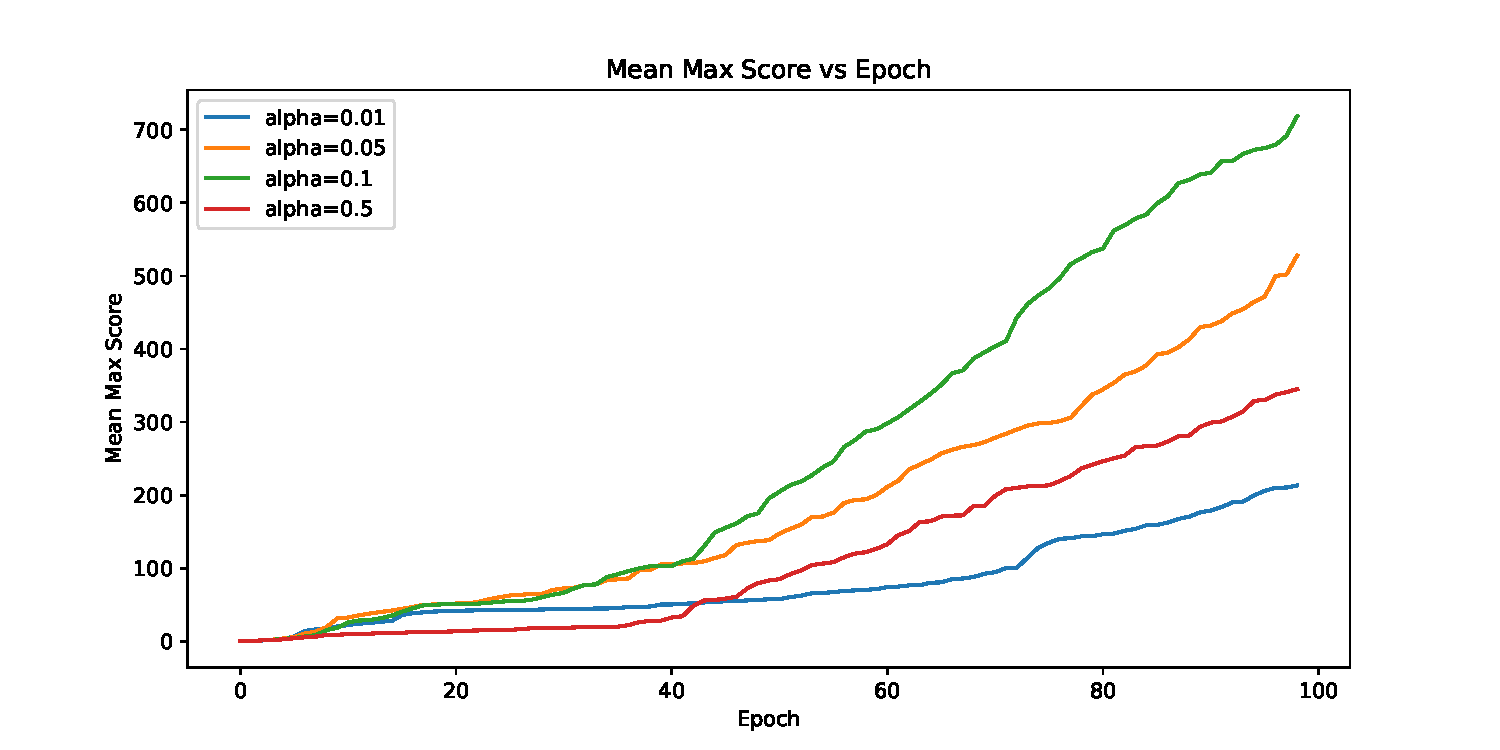
\includegraphics[scale=0.5]{figures/alpha_graph.pdf}
		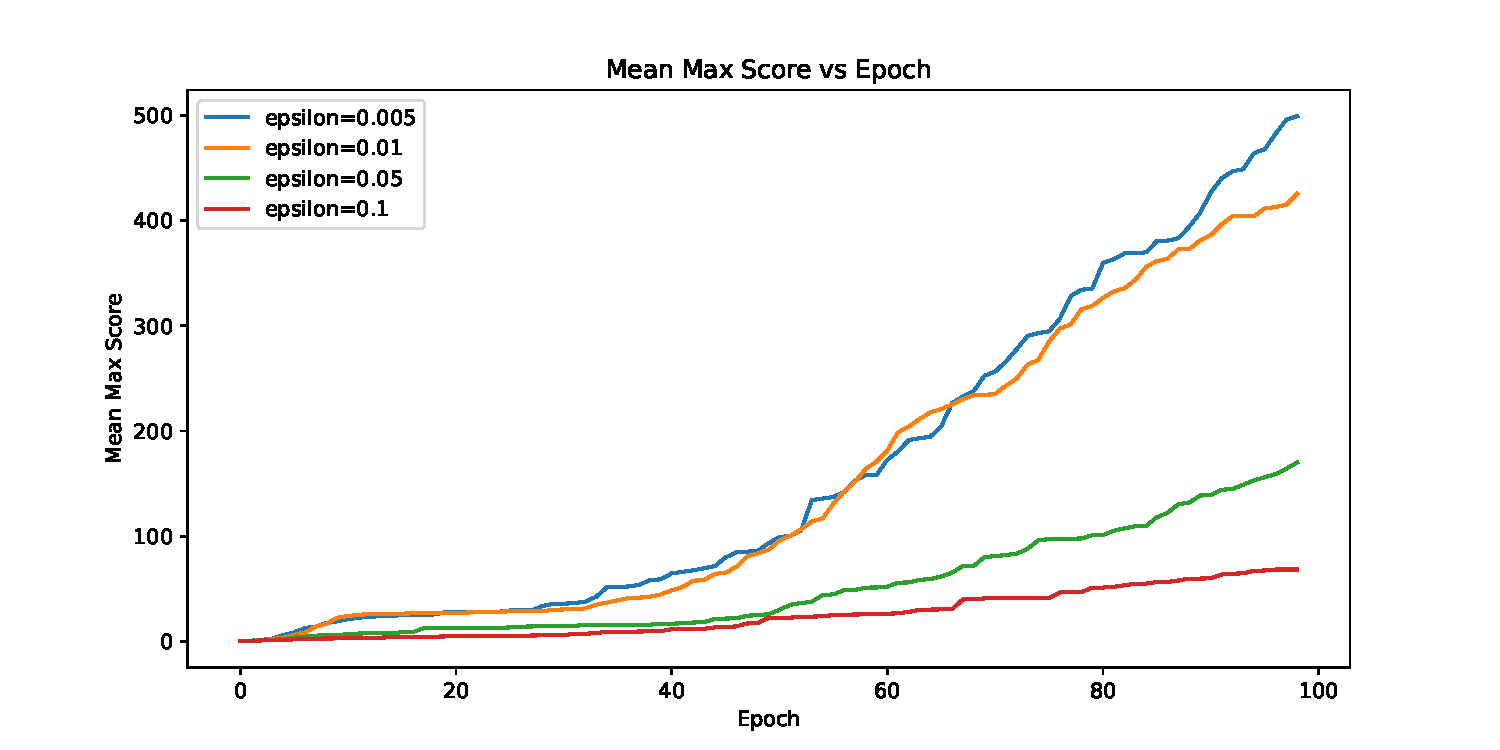
\includegraphics[scale=0.5]{figures/epsilon_graph.pdf}
	\end{center}


	Here is the code used to generate the data:
	\begin{minted}{python}
def mean_maxes(epsilon=0.01, alpha=0.5):
    epochs = 100

    hists = []
    for i in range(0, 100):
        agent = LearnerOptimized(epsilon=epsilon, alpha=alpha)
        hist = []
        run_games(agent, hist, epochs, 0)
        hists.append(hist)

    max_hists = [
        [max(hists[i][:n]) for n in range(1, epochs)] for i in range(0, len(hists))
    ]

    return [
        np.mean([max_hists[i][n] for i in range(0, len(hists))])
        for n in range(0, epochs - 1)
    ]
	\end{minted}
\end{parts}

\end{document}
